\documentclass[a4,12pt]{scrartcl}

%Basic 
\usepackage[utf8]{inputenc}
\usepackage[ngerman]{babel}
\usepackage[T1]{fontenc}
\usepackage{float}
%\usepackage[bottom = 3.50cm]{geometry}

%Titel Seite
\title{CLOUD INFRASTRUCTURE}
\subtitle{Lab-04}
\author{Giorgio Vincenti und Samuel Krieg}
\date{\today}


%Kopf, Fusszeile
\usepackage{fancyhdr}
\pagestyle{fancy}
\lhead{ \begin{picture}(0,0) \put(0,0){
\includegraphics[width=3cm]{./pictures/hsrlogo.png}} \end{picture}}
\chead{}
\rhead{Seite \thepage}
\lfoot{Cloud Infrastructure \\Lab-04}
\cfoot{Giorgio Vincenti und Samuel Krieg}
\rfoot{\today}
\renewcommand{\headrulewidth}{0.4pt}

%Bilder
\usepackage{graphicx}
\usepackage{wrapfig}

%Tabellen
\usepackage{booktabs}

%Codesnippets
\usepackage{listings}
\lstset{language=bash}  

%Querformat für eine Seite
\usepackage{lscape}
\usepackage{rotating}
\usepackage{pdflscape}

%Temp
\usepackage{lipsum}



\begin{document}

\clearpage\maketitle
\thispagestyle{empty}
\tableofcontents

\section{Aufgabenstellung}
Wurde aus der Aufgabenstellung entnommen:

Your teammate needs your help. She works in the software development team and is not really experienced in Linux server and virtualization. Create a How-to for your workmate in order that the software developer can use it.

What they need:
\begin{itemize}
\item 3 separated virtual machines
\item  VM1 has to be reachable from the internet and needs connectivity to VM2
\item VM2 needs connectivity to VM3
\item It has to be runnable on a virtual Linux server without GUI
\item Guess how long it will take for the SE
\end{itemize}

Add the following to your delivery:
\begin{itemize}
\item Usability
\item Is it possible to deploy the VMs on multiple hosts (2 Nodes)?
\end{itemize}

Hints
\begin{itemize}
\item Download Qcow image for VM
\item Qemu supports different network backend types
\item Guest VM don’t need a GUI
\end{itemize}

\subsection{Vorgehen}
\begin{itemize}
\item Ubuntu Server installiert

\item 
\begin{lstlisting}
sudo apt-get install
\end{lstlisting}
\end{itemize}
\subsection{Wichtiges im Überblick}
Hier einen Überblick über die erforderlichen Punkte:
\begin{itemize}
\item Anleitung für Software Engineering 
\begin{itemize}
\item Anleitung für erstellen / verwalten von VMs
\end{itemize}
\item 3 virtuelle Maschinen installieren
\item VM1 muss vom Internet aus erreichbar sein
\item VM2 muss mit VM3 kommunizieren können
\item Dauer einer Installation abschätzen / messen
\item Verwendbarkeit aufzeigen
\item Einsatz der VMs auf mehreren Hosts abklären
\end{itemize}

\subsection{Kriterien}
Wurden aus dem Mail von Urs Baumann entnommen: 
\begin{itemize}
\item Struktur
\item Verständlich für Software Entwickler
\item Funktionalität 
\item Kapitel zu Usability 
\item Eingesetzte Netzwerktypen 
\item Kapitel zu "multi host setup"  
\end{itemize}
\newpage

\section{Infrastruktur}
Hier einige Eckdaten zu der Infrastruktur. 

\subsection{Virtualisierungs-Software (Test-Umgebung)}
Um die Aufgabe durchzuführen wird die erforderliche Umgebung auf VMWare Workstation 12.0 aufgesetzt. 

\subsection{Virtualisierungs-Host}
Als Virtualisierungs-Host wir ein Linux OS eingsetzt. Wir gehen nicht auf die Details der Installation ein. Es wird nur das nötigste dokumentiert.  

\subsubsection{OS} 
Hier einige Details über die eingesetzte Linux Distribution. 
\begin{center}
    \begin{tabular}{@{} l l r@{}}\toprule    
    {Linux Distribution} & {Version}\\ \midrule
    Ubuntu & 14.04.3 LTS\\ \addlinespace
    \bottomrule
    \end{tabular}
\end{center}

\subsubsection{Login}
Um VMs auf dem Host erstellen zu können sind Berechtigungen erforderlich. Die Userin wird auf dem Host-Computer mit einem Administratorkonto arbeiten. 
\begin{center}
    \begin{tabular}{@{} l l r@{}}\toprule    
    {Benutzername} & {Passwort} & {Privilegien}\\ \midrule
    Cloud Infrastrucure & hsr12344 & Administrator (root)\\ \addlinespace
    \bottomrule
    \end{tabular}
\end{center}

\subsubsection{Network}
Der Host verfügt über eine statische IP-Konfiguration. Über diese IP kann der Server verwaltet werden. 
\begin{center}
    \begin{tabular}{@{} l l r@{}}\toprule    
    {Hostname} & {IP-Adresse} & {Subnetz}\\ \midrule
    Host & 10.0.1.11 & 255.255.255.0\\ \addlinespace
    \bottomrule
    \end{tabular}
\end{center}

\subsubsection{Services}
Auf dem Server laufen keine, für die Umgebung relevanten, Services. Es sind die Standard-Features von Ubuntu installiert.  

\subsubsection{Application}
Auf dem Ubuntu Client (Host) wird als Virtualisierungssoftware QEMU eingesetzt. Mit dieser Software soll die Anwendering VMs erstellen und verwalten können. 
\begin{center}
    \begin{tabular}{@{} l l r@{}}\toprule    
    {Software} & {Version}\\ \midrule
    QEMU emulator & 2.0.0\\ \addlinespace
    \bottomrule
    \end{tabular}
\end{center}
Die Installation der Software erfolgte über das Terminal: 
\begin{center}
    \begin{tabular}{@{} l l r@{}}\toprule    
    {Befehl} & {Bemerkung}\\ \midrule
    apt-get install qemu-system & Download und Installation\\
     \addlinespace
    \bottomrule
    \end{tabular}
\end{center}

\subsection{Virtualisierungs-Guests}
Die Umgebung besteht aus gesamt drei virtuellen Guests, die auf dem Virtualisierungs-Host laufen. Als Virtualisierungssoftware wird QEMU eingesetzt. 

\subsubsection{Guest-OS}
Als Guest-OS wird auf eine extrem kleine Linux Distribution gesetzt. Alle drei VMs betreiben dasselbe OS. 
\begin{center}
    \begin{tabular}{@{} l l r@{}}\toprule    
    {Distribution} & {Version} & {Hostname}\\ \toprule
    Tiny Core & v6.4 & vm1guest\\ 
    Tiny Core & v6.4 & vm2guest\\
    Tiny Core & v6.4 & vm3guest\\ \addlinespace
    \bottomrule
    \end{tabular}
\end{center}

\subsubsection{Guest-Path}
Die VMs befinden sich im Homeverzeichnis des Users. Sie sind als *.img Datei abgelegt.
\begin{center}
    \begin{tabular}{@{} l l r@{}}\toprule    
    {Image-Name} & {Path} & {Hostname}\\ \toprule
    vm1\_guest.img & /home/cldinf/Virtualdir & vm1guest\\ 
    vm2\_guest.img & /home/cldinf/Virtualdir & vm2guest\\
    vm3\_guest.img & /home/cldinf/Virtualdir & vm3guest\\ \addlinespace
    \bottomrule
    \end{tabular}
\end{center}

\begin{figure} [H]
	\begin{center}
	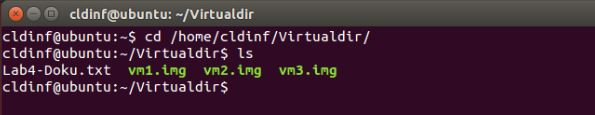
\includegraphics[width=0.80\textwidth]{./pictures/virtualdir.jpg}
	\caption{{Virtualdir Übersicht}}
	\label{virtualdir}
	\end{center}
\end{figure}

\subsection{Networking}
In diesem Kapitel werden einige Konfigurationsdetails zum Netzwerk aufgezeigt. 

\subsubsection{Host-Networkconfig}
Host IP Konfiguration und Tabs 

\subsubsection{Guest-Networkconfig}
Netzwerkkonfig von den Guests 

\subsubsection{Bridge}
Hier folgen die Daten der Bridge

\section{Anleitung}

\end{document}
